\documentclass[10pt]{article}
\usepackage{scrextend}
\changefontsizes{10.5pt}
\usepackage[margin=0.8in, top=0.7in, bottom=0.7in]{geometry}
\usepackage{graphicx}
\usepackage{natbib}
\usepackage{float}
\usepackage{amsmath}
\usepackage{amssymb}
\usepackage{hyperref}
\usepackage{booktabs}
\usepackage{caption}
\usepackage{subcaption}
\usepackage{enumitem}
\usepackage{wrapfig}
\usepackage{tikz}
\usetikzlibrary{arrows.meta, positioning, fit}

\setlist{nosep}
\captionsetup{font=small, skip=4pt}

% Compact sections
\usepackage{titlesec}
\titlespacing*{\section}{0pt}{1.2ex plus 0.3ex minus 0.2ex}{0.5ex plus 0.1ex}
\titlespacing*{\subsection}{0pt}{0.9ex plus 0.2ex minus 0.1ex}{0.3ex plus 0.1ex}
\titleformat{\section}{\normalfont\bfseries\normalsize}{\thesection}{0.6em}{}
\titleformat{\subsection}{\normalfont\bfseries\small}{\thesubsection}{0.5em}{}

%Tighter float / display spacing
\setlength{\parskip}{1pt plus 0.5pt}
\setlength{\textfloatsep}{7pt plus 1pt minus 1pt}
\setlength{\floatsep}{6pt plus 1pt minus 1pt}
\setlength{\intextsep}{6pt plus 1pt minus 1pt}
\setlength{\abovecaptionskip}{4pt}
\setlength{\belowcaptionskip}{2pt}
\setlength{\abovedisplayskip}{5pt plus 1pt minus 1pt}
\setlength{\belowdisplayskip}{5pt plus 1pt minus 1pt}


\makeatletter
\renewcommand{\maketitle}{\bgroup\setlength{\parindent}{0pt}
\begin{center}
  {\normalsize\bfseries Bayesian Heavy-Tailed Modeling of PM\textsubscript{2.5}\\[2pt]
   in British Columbia's Southern Interior\par}
  \vspace{5pt}
  {\small Eun Ji Hwang\\[1pt]}
  {\footnotesize STAT 405 Final Project --- Solo\\[1pt]
   Public repository: \url{https://github.com/eunji1120/UBC_Stat_405_project}\\[1pt]
   April 2026}
\end{center}\egroup\vspace{-0.5em}}
\makeatother

\begin{document}
\maketitle



\section{Introduction and Literature Review}

British Columbia (BC) has seen a dramatic increase in wildfire activity, with four of the most severe seasons of the past century occurring in 2017, 2018, 2021, and 2023 \citep{collins2025, daniels2024}. Climate change made the 2017 fire weather 2--4$\times$ more likely \citep{kirchmeier2018}, and the 2023 season set records with ${\sim}$2.84M hectares burned \citep{daniels2024}. The resulting smoke episodes push PM\textsubscript{2.5} to extreme levels, making robust statistical characterization of the tail behavior essential---particularly at stations lacking auxiliary chemical tracers.

Existing approaches to wildfire-influenced PM\textsubscript{2.5} modeling typically rely on external information: PM\textsubscript{2.5}/CO ratios \citep{jaffe2022}, trajectory-based classification with multi-station tracers \citep{schneider2021}, or CMAQ counterfactual simulations \citep{larsen2022}. Moreover, \citet{reid2021} showed that even machine learning models systematically under-predict extreme smoke days, suggesting that distributional assumptions themselves need attention. The most closely related work is \citet{schneider2021}, who analyzed multiple stations in western Canada with external tracers. Our work asks whether a single-station Bayesian heavy-tailed model, without any auxiliary information, can identify unusually extreme PM\textsubscript{2.5} behavior consistent with wildfire smoke---using the degrees-of-freedom parameter $\nu$ of a Student-$t$ likelihood as a data-driven measure of tail heaviness.

To this end, a Normal seasonal baseline is compared against a Student-$t$ model, and a Gaussian mixture is attempted (whose convergence failure is informative). Posteriors are computed via both HMC and ADVI, with critical evaluation of the approximation quality. Specifically, whether $\nu < 30$ (indicating heavy tails) and whether $\Delta\text{elpd}$ between the two models is practically significant has been tested.



\section{EDA (Exploratory Data Analysis)}

The dataset contains daily mean PM\textsubscript{2.5} from the Kamloops Federal Building station, located in BC's Southern Interior---a region frequently affected by wildfire smoke. The data span January 2022 to December 2025 ($N \approx 1{,}460$ days) and are drawn from the BC Air Data Archive.\footnote{\url{https://www.env.gov.bc.ca/epd/bcairquality/data/}} EDA was used to decide what kind of probability model is appropriate.

\paragraph{Distribution shape.} Because raw PM\textsubscript{2.5} is highly right-skewed, with spikes reaching $\sim 600\;\mu\mathrm{g}/\mathrm{m}^{3}$ during the 2023 wildfire season, first a log-transformation: $y_{t}=\log\left(\mathrm{PM}_{2.5, t}+0.1\right)$ was applied. Figure~\ref{fig:eda}a--b shows QQ-plots for the raw and transformed data. The raw data deviates strongly from normality in both tails. After transformation, the data follows the Normal reference line closely except in the upper tail. This suggests that after handling skewness, the main remaining departure from Normality is occasional extreme upper-tail behavior, motivating a Student-$t$ model. The histogram (Fig.~\ref{fig:eda}d) is unimodal, suggesting that these extremes may be better captured by a continuous heavy-tailed distribution than by a discrete second component, though this does not rule out mixture structure entirely.

\paragraph{Seasonality.} Because PM\textsubscript{2.5} levels also vary by month, seasonal effects have been included. The monthly boxplot (Fig.~\ref{fig:eda}c) shows elevated values from July to September, corresponding to the peak wildfire season.

\begin{figure}[H]
\centering
\begin{subfigure}[b]{0.235\textwidth}
    
\includegraphics[width=\textwidth]{figures/qq_raw.jpeg}
    \caption{QQ: raw}
\end{subfigure}\hfill
\begin{subfigure}[b]{0.235\textwidth}
    
\includegraphics[width=\textwidth]{figures/qq_log.jpeg}
    \caption{QQ: log}
\end{subfigure}\hfill
\begin{subfigure}[b]{0.235\textwidth}
    
\includegraphics[width=\textwidth]{figures/pm25_monthly_boxplot.jpeg}
    \caption{Monthly boxplot}
\end{subfigure}\hfill
\begin{subfigure}[b]{0.235\textwidth}
    
\includegraphics[width=\textwidth]{figures/pm25_histogram.jpeg}
    \caption{Histogram of $y_t$}
\end{subfigure}
\caption{(a) QQ-plot of raw PM$_{2.5}$ shows both tails are far from normal. (b) QQ-plot after log-transformation: skew is fixed but upper-tail deviation remains. (c) Monthly boxplots showing seasonal elevation from July to September. (d) Histogram of $y_t$: unimodal, no bimodal separation.}\label{fig:eda}
\end{figure}



\section{Models}

\noindent
\begin{minipage}[t]{0.60\textwidth}
\vspace{0pt}
The graphical model for the two specifications is shown in Figure~\ref{fig:dag}.
Model 1 has a normal observation distribution (no $\nu$ node), while Model 2 has a Student-$t$ distribution with learnt degrees of freedom $\nu$.

\subsection{Model 1: Normal Seasonal Baseline}
Model~1 is the starting point. It assumes that there are seasonal changes every month and that all variations are normally distributed. The mean for the whole year is $\mu$, the offset for each month is $\beta_m$ ($m = 1,\dots,12$), and the residual scale is $\sigma$.
\end{minipage}\hfill
\begin{minipage}[t]{0.37\textwidth}
\vspace{0pt}
\centering
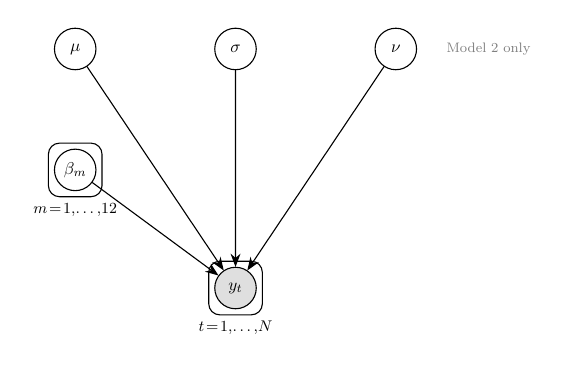
\begin{tikzpicture}[
    scale=0.62, every node/.style={scale=0.62},
    node distance=0.7cm,
    obs/.style={circle, draw, fill=gray!25, minimum size=0.85cm, inner sep=0pt},
    lat/.style={circle, draw, minimum size=0.85cm, inner sep=0pt},
    plate/.style={draw, rounded corners, inner sep=8pt},
    >=Stealth
]
\node[lat] (mu) {$\mu$};
\node[lat, right=1.5cm of mu] (sigma) {$\sigma$};
\node[lat, right=1.5cm of sigma] (nu) {$\nu$};
\node[lat, below=1.0cm of mu] (beta) {$\beta_m$};
\node[obs, below=2.5cm of sigma] (y) {$y_t$};
\draw[->] (mu) -- (y);
\draw[->] (sigma) -- (y);
\draw[->] (nu) -- (y);
\draw[->] (beta) -- (y);
\node[plate, fit=(beta)] (pbeta) {};
\node[below=0pt of pbeta, font=\small] {$m\!=\!1,\!\dots,\!12$};
\node[plate, fit=(y)] (py) {};
\node[below=0pt of py, font=\small] {$t\!=\!1,\!\dots,\!N$};
\node[right=0.3cm of nu, text=gray, font=\footnotesize] {Model~2 only};
\end{tikzpicture}
\captionof{figure}{Graphical model. Shaded = observed. $\nu$ node present only in Model~2.}\label{fig:dag}
\end{minipage}

\vspace{0.3em}
\vspace{-0.3em}
\[
\mu \sim \text{Normal}(2, 1),\quad \beta_m \sim \text{Normal}(0, 1),\quad \sigma \sim \text{Exp}(1), \quad y_t \sim \text{Normal}(\mu + \beta_{\text{month}[t]}, \sigma)
\]
\vspace{-0.6em}

\noindent A soft sum-to-zero constraint $\sum_m \beta_m \approx 0$ is applied so that $\mu$ can be interpreted as the grand mean. The prior on $\mu$ is centered at the median of $y_t$, and we use $\text{Exp}(1)$ on $\sigma$ which is weakly informative.

\subsection{Model 2: Student-$t$ Seasonal}
Model~2 has the same seasonal structure but uses the Student-$t$ distribution to capture heavier tails. The extra parameter $\nu$ (degrees of freedom) controls how heavy the tails are: a smaller $\nu$ gives more probability to extreme observations, and when $\nu \to \infty$ it reduces to Model~1.
\vspace{-0.3em}
\[
\nu \sim \text{Gamma}(2, 0.1), \quad y_t \sim \text{Student-}t(\nu,\; \mu + \beta_{\text{month}[t]},\; \sigma)
\]
\vspace{-0.6em}

\noindent with the same priors on $\mu$, $\beta_m$, $\sigma$. A $\text{Gamma}(2, 0.1)$ prior is used on $\nu$ (mean 20), which is weakly informative; prior predictive checks show that it puts almost no mass on $\nu < 2$ while still allowing both moderate ($\nu \sim 5$--$10$) and near-Normal tails. To check robustness, $\nu \sim \text{Exp}(0.1)$ and $\nu \sim \text{Gamma}(4, 0.2)$ are also fitted (Section~\ref{sec:results}).

Posterior means are reported as point estimates (the Bayes estimator under squared loss), along with posterior medians for $\nu$ since it is right-skewed (the Bayes estimator under absolute loss), and 90\% quantile-based credible intervals.\footnote{A natural hierarchical extension would set $\beta_m \sim \text{Normal}(0, \tau)$ with $\tau \sim \text{Half-Cauchy}(0, 1)$. Since there are ${\sim}120$ observations per month, sensitivity analysis shows that the posterior is not sensitive to the prior on $\beta_m$, so independent priors are used.} The Stan code with \texttt{generated quantities} blocks for LOO-CV and posterior predictive checks is in Appendix~\ref{app:stan}.



\section{Posterior Computation}

\subsection{Two Methods}
To assess whether a faster approximation changes the conclusions, both models were fit with two methods: (A)~Stan HMC/NUTS (4 chains, 1K warmup + 2K sampling) and (B)~Stan ADVI (meanfield, 1K samples). HMC explores the posterior via Hamiltonian dynamics and is the more reliable sampler here. ADVI is a faster alternative that approximates the posterior with a factorized Gaussian $q_\phi(x) = \prod_i \mathcal{N}(x_i;\, \mu_i, \sigma_i^2)$, minimizing the reverse KL divergence $\text{KL}(q_\phi \| \pi)$. This factorization may not work well for constrained or skewed parameters like $\nu$.

\subsection{Diagnostics}
HMC converged well for both main models, with stronger sampling efficiency for the Student-$t$ model. For Model~1, $\hat{R} \leq 1.01$ for all parameters. The bulk ESS for $\mu$ and $\beta_m$ is 370--384, which is modest due to the $\mu$-$\beta$ tradeoff; however, $\hat{R}$ remains low, MCSE for $\mu$ is 0.015, and there are no divergent transitions, so the sampler has converged despite the slower mixing. For Model~2, $\hat{R} = 1.00$ with bulk ESS $> 3{,}700$ and MCSE $< 0.012$ for all parameters, including $\nu$, with no divergent transitions. Full summaries with trace plots are in Appendix~\ref{app:diag}.

\subsection{Correctness Validation}
To verify that the inference procedure was calibrated, a synthetic-data experiment has been run: for 50 replications, parameters from the Model~2 prior were drawn, simulated $N=200$ observations, ran HMC, and checked 90\% credible interval coverage. Coverage was satisfactory for $\sigma$ (96\%) and $\nu$ (92\%), but weaker for $\mu$ (76\%). This under-coverage reflects the $\mu$-$\beta_m$ tradeoff: because these are only softly identified via the sum-to-zero constraint, $\mu$ may exhibit under-coverage even when the fitted monthly means $\mu + \beta_m$ are well-calibrated (verified to achieve 90\% coverage). Therefore, inference is more reliable for fitted monthly means than for $\mu$ alone (Appendix~\ref{app:synth}).



\section{Results}\label{sec:results}

\subsection{Posterior Summaries}
The main result is that the Student-$t$ model shows substantial tail heaviness: $\hat{\nu} = 6.70$ (90\% CI: $[5.45, 8.23]$, median 6.61), which is well below 30. A low $\nu$ means the distribution gives more probability to extreme values than a Normal would. Model~2's scale $\hat{\sigma} = 0.578$ is lower than Model~1's 0.691: the inflated $\sigma$ in Model~1 was absorbing the extremes that Model~2 handles through heavy tails.

Seasonal effects are consistent across models but estimated with much better precision under Model~2 (posterior SDs ${\sim}0.04$ vs ${\sim}0.29$). This is since the Student-$t$ reduces the influence of extreme observations on the seasonal mean estimates, which leads to tighter credible intervals.

\begin{table}[H]
\centering\small
\caption{Posterior comparison: Model 1 (Normal) vs Model 2 (Student-$t$).}\label{tab:comparison}
\begin{tabular}{lcccc}
\toprule
 & \multicolumn{2}{c}{Model 1 (Normal)} & \multicolumn{2}{c}{Model 2 (Student-$t$)} \\
\cmidrule(lr){2-3}\cmidrule(lr){4-5}
Parameter & Mean [90\% CI] & ESS & Mean [90\% CI] & ESS \\
\midrule
$\mu$     & 1.93 [1.43, 2.42] & 374  & 1.92 [1.90, 1.95] & 12058 \\
$\beta_8$ (Aug) & 0.38 [$-$0.20, 0.95] & 380  & 0.33 [0.26, 0.41] & 10393 \\
$\beta_9$ (Sep) & 0.41 [$-$0.17, 0.98] & 378  & 0.37 [0.29, 0.45] & 9094 \\
$\sigma$  & 0.691 [0.675, 0.707] & 1269 & 0.578 [0.555, 0.601] & 6144 \\
$\nu$     & --- & --- & 6.70 [5.45, 8.23] & 6065 \\
\midrule
LOO elpd  & \multicolumn{2}{c}{baseline} & \multicolumn{2}{c}{$+57.7$ (SE $= 14.8$)} \\
\bottomrule
\end{tabular}
\end{table}

\subsection{Model Comparison}

\noindent
\begin{minipage}[t]{0.63\textwidth}
\vspace{0pt}
\paragraph{LOO-CV.} Model~2 is strongly favored: $\Delta\text{elpd} = 57.7$ (SE $= 14.8$), which is ${\sim}3.9$ standard errors. This means the Student-$t$ model predicts unseen data much better than the Normal model. All Pareto-$\hat{k}$ values are below 0.7, which shows that the LOO-CV estimates from the \texttt{loo} R package are reliable.

\paragraph{Posterior predictive check.} Since the main modeling challenge is the extreme upper-tail events, whether each model can reproduce the observed maximum is checked. The distribution of $\max(y_{\text{rep}})$ (Fig.~\ref{fig:ppc}) shows that Model~1 almost never generates values as large as the observed maximum, while Model~2 covers it well.
\end{minipage}\hfill
\begin{minipage}[t]{0.24\textwidth}
\vspace{0pt}
\centering

\includegraphics[width=0.85\textwidth]{figures/ppc_max.jpeg}
\captionof{figure}{PPC: $\max(y_{\text{rep}})$. Dashed line = observed max. Model~1 fails; Model~2 succeeds.}\label{fig:ppc}
\end{minipage}

\vspace{0.3em}

\paragraph{HMC vs ADVI.} This comparison checks whether a fast variational approximation would give the same conclusion. It does not: ADVI places mass around $\nu \approx 60$, which effectively makes it a Normal-like model, and compensates by inflating $\sigma$ to ${\sim}1.35$ (vs HMC's 0.58). This happens since the factorized Gaussian family cannot capture the skewness or lower bound of the posterior of $\nu$ (Appendix~\ref{app:ppc}, Fig.~\ref{fig:hmc_advi}). This shows that HMC is necessary for reliable inference when the posterior has non-Gaussian structure.

\paragraph{Prior sensitivity.} Since the tail parameter $\nu$ is central to the analysis, whether the result depends on its prior is also checked. All three priors---$\text{Gamma}(2, 0.1)$, $\text{Exp}(0.1)$, and $\text{Gamma}(4, 0.2)$---give $\hat{\nu} \in [6.5, 7.0]$ with overlapping 90\% CIs (Appendix~\ref{app:sensitivity}), which confirms the posterior is data-driven.

\paragraph{Mixture model attempt.} A two-component Gaussian mixture (Appendix~\ref{app:mixture}) is also attempted as an exploratory check. Under this specification, the mixture did not produce a reliable fit ($\hat{R} = 1.73$, ESS $\approx 6$) even with ordering constraints and tuning, which suggests the data do not strongly support two discrete regimes.


\section{Discussion}\label{sec:discussion}

Daily log-PM\textsubscript{2.5} in Kamloops exhibits heavy tails that a Normal model cannot capture. The posterior $\hat{\nu} \approx 6.7$ is well below the threshold at which the Student-$t$ is practically indistinguishable from a Normal, the LOO-CV ($\Delta\text{elpd} = 57.7$) strongly favors the Student-$t$, and the posterior predictive check confirms that only the Student-$t$ can reproduce the observed extreme. This is consistent with wildfire smoke creating occasional severe spikes that do not form a separate population but instead thicken the upper tail. From a predictive standpoint, the Student-$t$ model would assign materially higher probability to future extreme smoke events than the Normal baseline, which is important for risk assessment.

The ADVI comparison also shows an important point: mean-field variational inference fails for the bounded, skewed posterior of $\nu$, which gives estimates that effectively go back to a Normal model. Since the reverse KL penalizes $q$ for placing mass where $\pi$ is small but not the other way around, the mean-field approximation avoids the low-$\nu$ region (where the true posterior concentrates) and instead spreads toward larger $\nu$ values where $q$ has less penalty.

\paragraph{Limitations.} Both models assume conditional independence given the month; an AR(1) extension ($y_t = \mu + \beta_{\text{month}[t]} + \epsilon_t$, \; $\epsilon_t = \phi\,\epsilon_{t-1} + w_t$, \; $w_t \sim \text{Student-}t(\nu,0,\sigma)$, \; $\phi \sim \text{Uniform}(-1,1)$) would address the observed lag-1 ACF $\approx 0.3$ but was not pursued as it requires a fundamentally different Stan implementation; consequently, posterior uncertainty for seasonal effects may be underestimated. Additionally, results are from a single station. A quick check with log-offset $c \in \{0.01, 0.1, 1.0\}$ yielded $\hat{\nu} \in [6.4, 7.1]$, suggesting moderate robustness to this choice. Finally, the Student-$t$ model provides a continuous measure of tail heaviness rather than an explicit smoke-day classification.

\paragraph{Broader context and future work.} Even without tracer data, a single-station heavy-tailed seasonal model provides a continuous, uncertainty-quantified summary of extreme PM\textsubscript{2.5} tail behavior via $\nu$, avoiding binary smoke classification. Future work could incorporate autoregressive structure to address the independence limitation, extend to multiple stations, or combine Student-$t$ tails with mixture components---a direction suggested by the purely Gaussian mixture's convergence failure.

\newpage
\bibliographystyle{apalike}
\bibliography{references}


\newpage
\appendix


\section{Stan Code}\label{app:stan}

\subsection*{Model 1: Normal Seasonal Baseline}
\begin{verbatim}
data {
  int<lower=0> N;
  vector[N] y;
  array[N] int<lower=1, upper=12> month;
}
parameters {
  real mu;
  vector[12] beta;
  real<lower=0> sigma;
}
model {
  mu ~ normal(2, 1);
  beta ~ normal(0, 1);
  sigma ~ exponential(1);
  sum(beta) ~ normal(0, 0.001);
  for (n in 1:N)
    y[n] ~ normal(mu + beta[month[n]], sigma);
}
generated quantities {
  vector[N] log_lik;
  vector[N] y_rep;
  for (n in 1:N) {
    log_lik[n] = normal_lpdf(y[n] | mu + beta[month[n]], sigma);
    y_rep[n] = normal_rng(mu + beta[month[n]], sigma);
  }
}
\end{verbatim}

\subsection*{Model 2: Student-$t$ Seasonal}
\begin{verbatim}
data {
  int<lower=0> N;
  vector[N] y;
  array[N] int<lower=1, upper=12> month;
}
parameters {
  real mu;
  vector[12] beta;
  real<lower=0> sigma;
  real<lower=1> nu;
}
model {
  mu ~ normal(2, 1);
  beta ~ normal(0, 1);
  sigma ~ exponential(1);
  nu ~ gamma(2, 0.1);
  sum(beta) ~ normal(0, 0.001);
  for (n in 1:N)
    y[n] ~ student_t(nu, mu + beta[month[n]], sigma);
}
generated quantities {
  vector[N] log_lik;
  vector[N] y_rep;
  for (n in 1:N) {
    log_lik[n] = student_t_lpdf(y[n] | nu, mu+beta[month[n]], sigma);
    y_rep[n] = student_t_rng(nu, mu+beta[month[n]], sigma);
  }
}
\end{verbatim}

\section{HMC vs ADVI Comparison}\label{app:ppc}

\begin{verbatim}
fit2_vi <- mod2$variational(
  data = stan_data,
  algorithm = "meanfield",
  output_samples = 1000
)
\end{verbatim}

\begin{figure}[H]
\centering
\begin{subfigure}[b]{0.48\textwidth}
    
\includegraphics[width=\textwidth]{figures/hmc_vs_advi_nu.jpeg}
    \caption{$\nu$: ADVI $\approx 60$, HMC $\approx 7$}
    \label{fig:advi_nu}
\end{subfigure}\hfill
\begin{subfigure}[b]{0.48\textwidth}
    
\includegraphics[width=\textwidth]{figures/hmc_vs_advi_sigma.jpeg}
    \caption{$\sigma$: ADVI $\approx 1.35$, HMC $\approx 0.58$}
    \label{fig:advi_sigma}
\end{subfigure}
\caption{HMC vs ADVI for Model~2.}\label{fig:hmc_advi}
\end{figure}

\section{Diagnostics}\label{app:diag}

\begin{table}[H]
\centering\small
\caption{Model 1 posterior summary with MCSE.}
\begin{tabular}{lrrrrrr}
\toprule
Parameter & Mean & SD & MCSE & $\hat{R}$ & ESS (bulk) & ESS (tail) \\
\midrule
$\mu$     & 1.930 & 0.287 & 0.015 & 1.01 &  374 &  397 \\
$\beta_7$ & 0.175 & 0.291 & 0.015 & 1.01 &  382 &  444 \\
$\beta_8$ & 0.377 & 0.291 & 0.015 & 1.01 &  380 &  425 \\
$\beta_9$ & 0.409 & 0.292 & 0.015 & 1.01 &  378 &  407 \\
$\sigma$  & 0.691 & 0.009 & 0.0003& 1.00 & 1269 & 1480 \\
\bottomrule
\end{tabular}
\end{table}

\begin{figure}[H]
\centering

\includegraphics[width=0.75\textwidth]{figures/model1_traceplot.jpeg}
\caption{Model 1 trace plots.}
\end{figure}

\begin{table}[H]
\centering\small
\caption{Model 2 posterior summary with MCSE.}
\begin{tabular}{lrrrrrr}
\toprule
Parameter & Mean & SD & MCSE & $\hat{R}$ & ESS (bulk) & ESS (tail) \\
\midrule
$\mu$     & 1.920 & 0.013 & 0.0001 & 1.00 & 12058 & 6003 \\
$\beta_7$ & 0.134 & 0.044 & 0.0004 & 1.00 & 10365 & 5775 \\
$\beta_8$ & 0.333 & 0.046 & 0.0005 & 1.00 & 10393 & 4967 \\
$\beta_9$ & 0.370 & 0.048 & 0.0005 & 1.00 &  9094 & 6044 \\
$\sigma$  & 0.578 & 0.014 & 0.0002 & 1.00 &  6144 & 5772 \\
$\nu$     & 6.700 & 0.868 & 0.011  & 1.00 &  6065 & 5758 \\
\bottomrule
\end{tabular}
\end{table}

\begin{figure}[H]
\centering

\includegraphics[width=0.75\textwidth]{figures/model2_traceplot.jpeg}
\caption{Model 2 trace plots. Excellent mixing.}
\end{figure}



\section{Synthetic Data Calibration}\label{app:synth}

50 datasets from the Model~2 prior was simulated, HMC has been run on each, and whether the 90\% credible intervals achieved nominal coverage has been checked.

\begin{table}[H]
\centering\small
\caption{Synthetic data coverage rates (nominal 90\%, 50 replications).}
\begin{tabular}{lr}
\toprule
Parameter & Coverage (\%) \\
\midrule
$\mu$    & 76  \\
$\sigma$ & 96 \\
$\nu$    & 92 \\
\bottomrule
\end{tabular}
\end{table}

The under-coverage for $\mu$ is due to the $\mu$-$\beta_m$ tradeoff: since these two parameters are only softly identified through the sum-to-zero constraint, $\mu$ can show under-coverage even when the fitted values $\mu + \beta_m$ are well-calibrated. The main point is that the inference procedure is calibrated for the quantities that are actually interpreted---namely $\sigma$, $\nu$, and the monthly means---even though $\mu$ alone has wider variation.


\section{Prior Sensitivity Analysis}\label{app:sensitivity}

\begin{table}[H]
\centering\small
\caption{Prior sensitivity for $\nu$.}\label{tab:sensitivity}
\begin{tabular}{lrrr}
\toprule
Prior on $\nu$ & Post.\ Mean & Post.\ Median & 90\% CI \\
\midrule
$\text{Gamma}(2, 0.1)$ [baseline] & 6.70 & 6.61 & $[5.45, 8.23]$ \\
$\text{Exp}(0.1)$                  & 6.58 & 6.50 & $[5.40, 8.08]$ \\
$\text{Gamma}(4, 0.2)$            & 6.85 & 6.75 & $[5.54, 8.46]$ \\
\bottomrule
\end{tabular}
\end{table}


\section{Mixture Model Attempt}\label{app:mixture}

A two-component Gaussian mixture with month-varying weights and $\mu_1 = \mu_0 + \delta$ ($\delta > 0$) is also attempted as an exploratory check. Even with $\delta \sim \operatorname{Lognormal}(0, 0.5)$ and \texttt{adapt\_delta} $= 0.95$, all runs showed $\hat{R} = 1.73$ and bulk ESS $\approx 6$, with chains getting stuck in separate modes. This means the mixture did not produce a reliable fit, which suggests that the data do not strongly support two discrete regimes. However, a different mixture parameterization might work better.

\begin{verbatim}
data {
  int<lower=0> N;
  vector[N] y;
  array[N] int<lower=1, upper=12> month;
}
parameters {
  real mu0;
  real<lower=0> delta;
  real<lower=0> sigma0;
  real<lower=0> sigma1;
  vector[12] alpha;
}
transformed parameters {
  real mu1 = mu0 + delta;
}
model {
  mu0 ~ normal(1.5, 0.5);
  delta ~ lognormal(0, 0.5);
  sigma0 ~ exponential(1);
  sigma1 ~ exponential(1);
  alpha ~ normal(0, 1);
  for (n in 1:N) {
    real lp = log_inv_logit(alpha[month[n]]);
    real l1mp = log1m_inv_logit(alpha[month[n]]);
    target += log_sum_exp(
      lp + normal_lpdf(y[n] | mu1, sigma1),
      l1mp + normal_lpdf(y[n] | mu0, sigma0));
  }
}
\end{verbatim}

\begin{table}[H]
\centering\small
\caption{Mixture model posterior summary.}
\begin{tabular}{lrrrrr}
\toprule
Parameter & Mean & SD & $\hat{R}$ & ESS (bulk) & ESS (tail) \\
\midrule
$\mu_0$    & 1.820 & 0.056 & 1.73 & 6.1 & 116 \\
$\delta$   & 0.259 & 0.255 & 1.73 & 6.1 & 117 \\
$\sigma_0$ & 0.795 & 0.239 & 1.73 & 6.1 & 116 \\
$\sigma_1$ & 0.726 & 0.195 & 1.73 & 6.1 & 119 \\
\bottomrule
\end{tabular}
\end{table}

\begin{figure}[H]
\centering
\includegraphics[width=0.75\textwidth]{figures/mixture_traceplot.jpeg}
\caption{Mixture trace plots: chains stuck in separate modes.}
\end{figure}


\section{AI Usage Disclosure}

AI tools were used in the following limited capacities during this project:

\begin{enumerate}
    \item \textbf{Code debugging.} When encountering errors in R or Stan code, I described the error message and my intended logic to Claude and asked it to help identify the bug. I reviewed each suggestion and decided whether to apply it.
    \item \textbf{Text editing.} Grammarly was used for grammar correction. Both Grammarly and Claude were used to condense paragraphs to meet the page limit, after which I reviewed and further edited the output myself.
\end{enumerate}

\end{document}